\section*{}
\begin{figure}[h]
    \centering
    \begin{subfigure}[t]{0.49\textwidth}
        \centering
        \includegraphics[width = \textwidth]{fig/total_debt.pdf}
        \caption{Top 30 Debtor by Total Debt in USD}
        \label{fig:total-debt-30}
    \end{subfigure}%
    ~
    \begin{subfigure}[t]{0.49\textwidth}
        \centering
        \includegraphics[width = \textwidth]{fig/perc_debt.pdf}
        \caption{Top 30 Debtor by Dept-to-GDP Ratio}
        \label{fig:perc-debt-30}
    \end{subfigure}
    \caption{Debt to China Statistic by Country in 2017}
    \label{fig:Country-Agg}
    \floatfoot{\emph{Source:} \citet*{Horn-Reinhart-Trebesch-21} database \\
    \emph{Note:} The figure on the left presents the top 30 countries in amount of total external debt to China in 2017. The figure on the right compares by the China-debt-to-GDP ratio.}
\end{figure}

\begin{figure}[h]
    \centering
    \includegraphics[width = 0.8\textwidth]{fig/aggr_debt_source.pdf}
    \caption{Change of Aggregate Public Debt for Different Official Creditors}
    \label{fig:debt-ts}
    \floatfoot{\emph{Source}: \citet*{Horn-Reinhart-Trebesch-21} database \\
    \emph{Note}: The figure shows the change in the aggregate external public debt that the developing countries owed to different official creditors. These include China, World Bank (excluding China), IMF, and all 22 Paris Club governments. It is obvious that China had become the largest official creditors in the world according to the estimation of \citet*{Horn-Reinhart-Trebesch-21}.}
\end{figure}

\begin{figure}[h]
    \centering
    \begin{subfigure}[position]{0.8\textwidth}
        \centering
        \includegraphics[width=\textwidth]{fig/ALL/Sri Lanka_debt_source.pdf}
        \caption{Sri Lanka}
        \label{fig: sri-lanka-debt-ts}
    \end{subfigure}
    \begin{subfigure}[position]{0.8\textwidth}
        \centering
        \includegraphics[width = \textwidth]{fig/ALL/Pakistan_debt_source.pdf}
        \caption{Pakistan}
        \label{fig: pakistan-debt-ts}
    \end{subfigure}
    \caption{Debt to Main Creditors}
    \label{fig: LAK-PAK-debt-ts}
    \floatfoot{\emph{Source:} \citet*{Horn-Reinhart-Trebesch-21} database \\
    \emph{Note:} The figure shows the change in the external public debt that Sri Lanka and Pakistan owed to different official creditors. These include China, World Bank (excluding China), IMF, and all 22 Paris Club governments.}
\end{figure}

            %%%%%%%%%%%%%%%%%%%%%%%%%%%%%%%%%%%%
            % Decompose Tradable HP
            %%%%%%%%%%%%%%%%%%%%%%%%%%%%%%%%%%%%
\begin{figure}[h]
    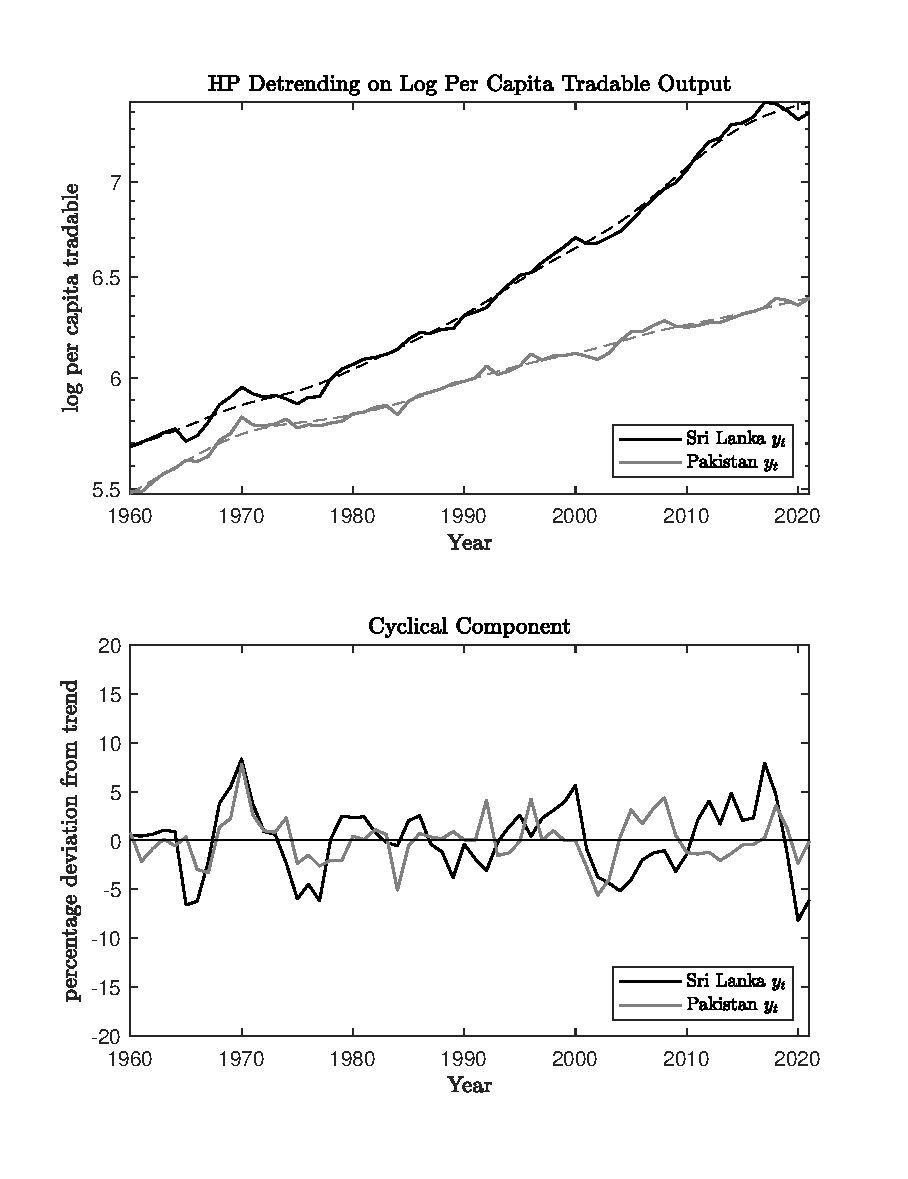
\includegraphics[width = \textwidth]{fig/decompose_trad_hp.eps}
    \caption{Decomposition of log-real-tradable-GDP for Sri Lanka and Pakistan Using HP-Filter}
    \label{fig:decompose-trad-hp}
    \floatfoot{\emph{Source:} World Bank national accounts data. \\
    \emph{Note:} The cyclical component in the right is obtained by the HP-filter with smoothing parameter $\lambda = 100$ for the log-real-GDP in the left. The quarterized AR(1) estimation for Sri Lanka yields $(\rho, \sigma_u)= (0.9114, 0.0180)$, and for Pakistan yields $(\rho, \sigma_u)= (0.8518, 0.0116)$}
\end{figure}

            %%%%%%%%%%%%%%%%%%%%%%%%%%%%%%%%%%%%
            % Decompose Tradable Log-Q
            %%%%%%%%%%%%%%%%%%%%%%%%%%%%%%%%%%%%
\begin{figure}[h]
    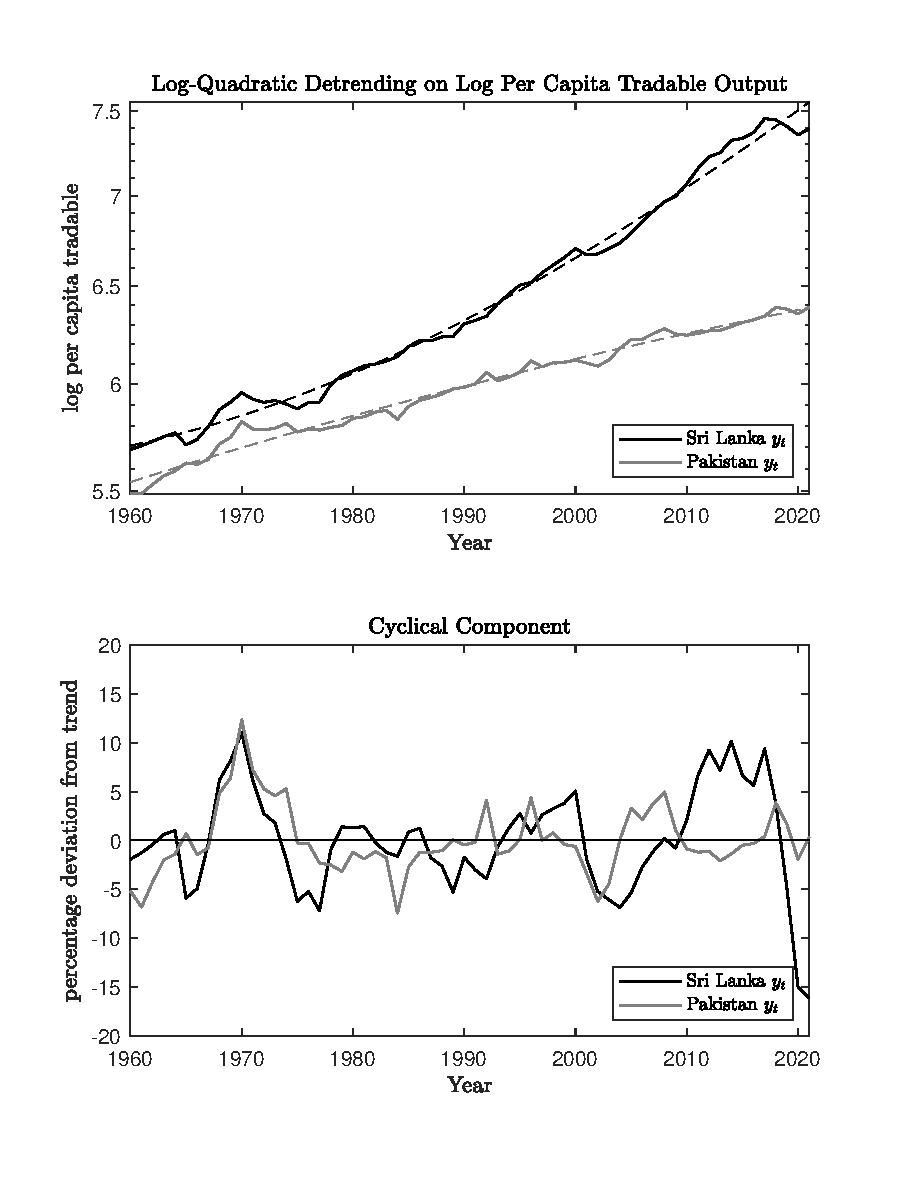
\includegraphics[width = \textwidth]{fig/decompose_trad_logq.eps}
    \caption{Decomposition of log-real-tradable-GDP for Sri Lanka and Pakistan Using Log-quadratic Filter}
    \label{fig:decompose-trad-logq}
    \floatfoot{\emph{Source:} World Bank national accounts data. \\
    \emph{Note:} The cyclical component in the right is obtained by the log-quadratic filter for the log-real-GDP in the left. The quarterized AR(1) estimation for Sri Lanka yields $(\rho, \sigma_u)= (0.9325, 0.0266)$, and for Pakistan yields $(\rho, \sigma_u)= (0.9239, 0.0174)$}
\end{figure}


\begin{figure}
     \begin{subfigure}[t]{\textwidth}
        \includegraphics[width = \textwidth]{fig/sri_lanka_debt_gdp.pdf}
        \caption{Sri Lanka}
        \label{fig: sri_d_t_trad}
    \end{subfigure}

     \begin{subfigure}[t]{\textwidth}
        \includegraphics[width = \textwidth]{fig/pak_debt_gdp.pdf}
        \caption{Pakistan}
        \label{fig: pak_d_t_trad}
    \end{subfigure}
    \caption{Debt Stock, Tradable GDP, and the Ratio, 2007 -- 2017}
    \label{fig: d-t_trad}
    \floatfoot{\emph{Source:} Debt data from IDS Database and \citet*{Horn-Reinhart-Trebesch-21} Database. GDP data from World Bank.\\
        \emph{Note:} The figure shows the change of total debt level versus the nominal GDP for tradable goods, defined as the sum of agriculture, forestry, fishing, and industry. The left vertical axis represents the values of debts and nominal tradable-GDP in billion USD, depicted by solid lines. The right vertical axis corresponds to the ratio shown as a dashed black line, reflecting the ratio of debt-to-tradable-GDP.
    }
\end{figure}
%https://www.bbc.com/news/world-south-asia-11060119

\begin{figure}[t]
    \centering
    \begin{subfigure}[t]{0.8\textwidth}
        \centering
        \includegraphics[width = \textwidth]{fig/default_set_sri_trad_hp.eps}
        \caption{Sri Lanka}
        \label{fig: ds-sri}
    \end{subfigure}%

    \begin{subfigure}[t]{0.8\textwidth}
        \centering
        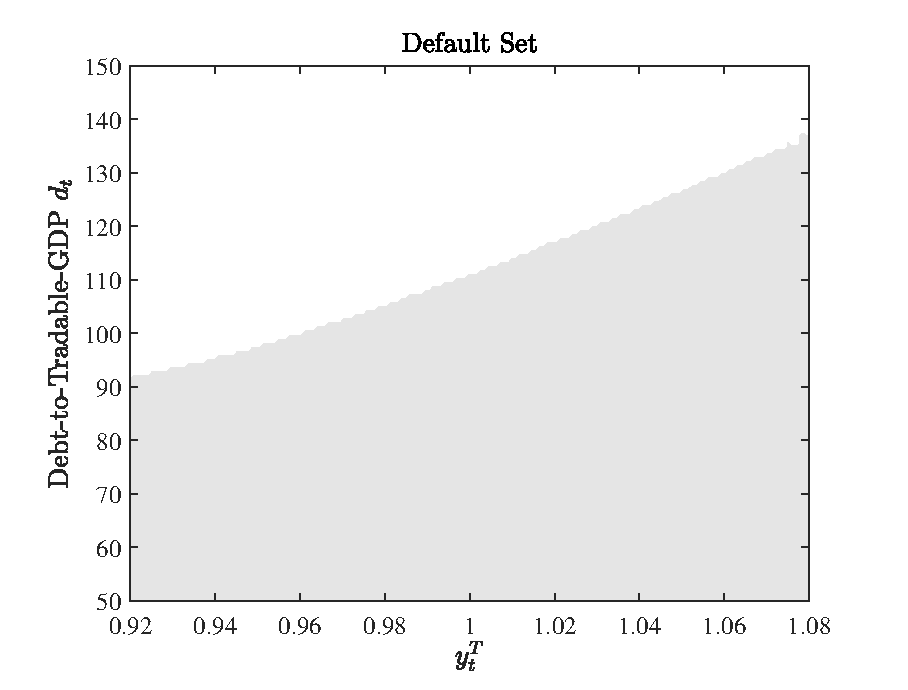
\includegraphics[width = \textwidth]{fig/default_set_pak_trad_hp.eps}
        \caption{Pakistan}
        \label{fig: ds-pak}
    \end{subfigure}
    \caption{Graphical Representation of Default Set}
    \label{fig:ds}
    \floatfoot{\emph{Note:} The default set derived via value function iteration is plotted on the state space. The horizontal axis represents the tradable output level, and the vertical axis represents the debt stock. The gray area represents the grid point where the country chooses not to default, and the white area is the grid point where default is the optimal action for the country.}
\end{figure}



\begin{figure}
    \begin{subfigure}[t]{0.8\textwidth}
        \includegraphics[width = \textwidth]{fig/default_set_sri_trad_hp_with_china.eps}
        \caption{Debt to All Creditors}
        \label{fig: ds-sri-data-with-china}
    \end{subfigure}

    \begin{subfigure}[t]{0.8\textwidth}
        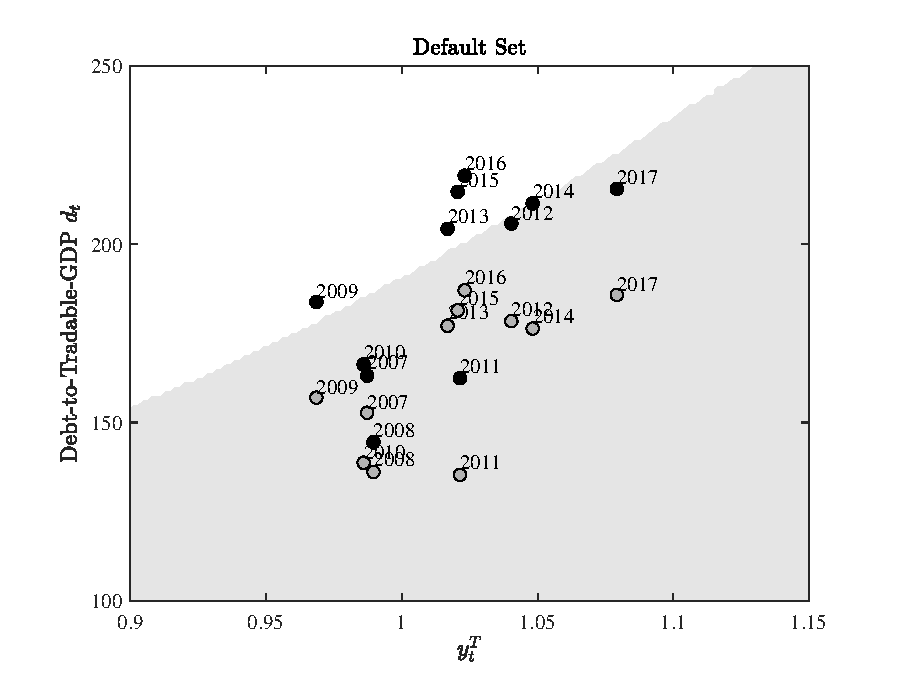
\includegraphics[width = \textwidth]{fig/default_set_sri_trad_hp_x_china.eps}
        \caption{Excluding Debt to China}
        \label{fig: ds-sri-data-x-china}
    \end{subfigure}
    \caption{Mapping Actual Data onto Analytical Model for Sri Lanka, 2007 -- 2017}
    \label{fig:ds-sri-data}
    \floatfoot{\emph{Source:} Debt data from IDS Database and \citet*{Horn-Reinhart-Trebesch-21} Database. GDP data from World Bank\\
        \emph{Note:} The gray region represents the non-default set of Sri Lanka, and the white region represents the default set. Black dots in (a) and (b) represents the output-debt pair in the real data, and the gray dots in (b) represents the output-debt pair that excludes the debts from China. Debt here corresponds to the unsecured debt amount per quarter.
    }
\end{figure}



\begin{figure}
    \begin{subfigure}[t]{0.8\textwidth}
        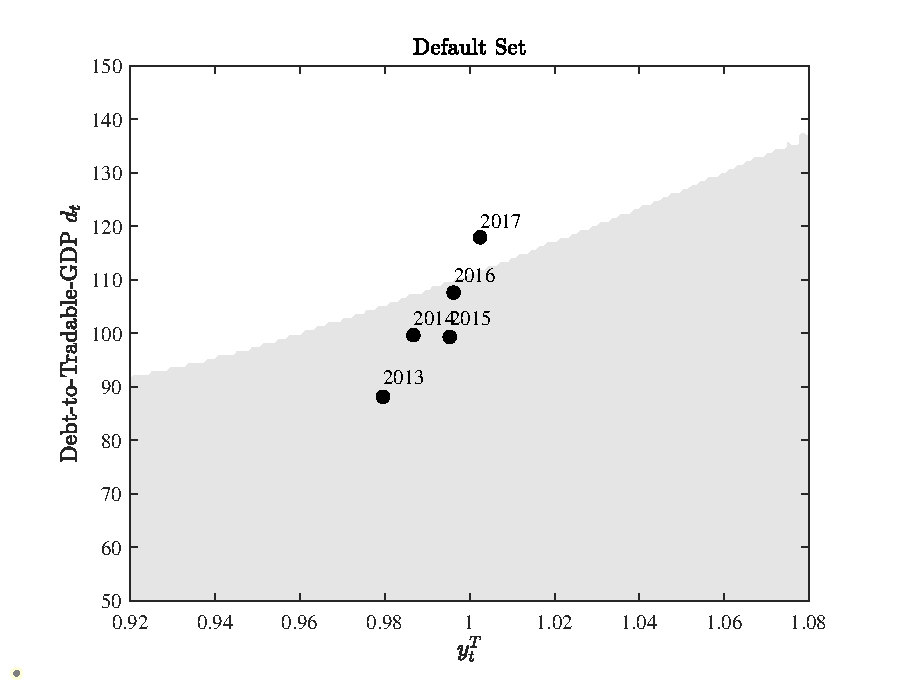
\includegraphics[width = \textwidth]{fig/default_set_pak_trad_hp_with_china.eps}
        \caption{Debt to All Creditors}
        \label{fig: ds-pak-data-with-china}
    \end{subfigure}

    \begin{subfigure}[t]{0.8\textwidth}
        \includegraphics[width = \textwidth]{fig/default_set_pak_trad_hp_x_china.eps}
        \caption{Excluding Debt to China}
        \label{fig: ds-pak-data-x-china}
    \end{subfigure}
    \caption{Mapping Actual Data onto Analytical Model for Pakistan, 2013 -- 2017}
    \label{fig:ds-pak-data}
    \floatfoot{\emph{Source:} Debt data from IDS Database and \citet*{Horn-Reinhart-Trebesch-21} Database. GDP data from World Bank\\
        \emph{Note:} The gray region represents the non-default set of Pakistan, and the white region represents the default set. Black dots in (a) and (b) represents the output-debt pair in the real data, and the gray dots in (b) represents the output-debt pair that excludes the debts from China. Debt here corresponds to the unsecured debt amount per quarter.
    }
\end{figure}


            %%%%%%%%%%%%%%%%%%%%%%%%
            % Using Log-Q
            %%%%%%%%%%%%%%%%%%%%%%%%
\begin{figure}
    \begin{subfigure}[t]{0.8\textwidth}
        \includegraphics[width = \textwidth]{fig/default_set_sri_trad_logq_with_china.eps}
        \caption{Sri Lanka}
        \label{fig: ds-sri-logq}
    \end{subfigure}

    \begin{subfigure}[t]{0.8\textwidth}
        \includegraphics[width = \textwidth]{fig/default_set_pak_trad_logq_with_china.eps}
        \caption{Pakistan}
        \label{fig: ds-pak-logq}
    \end{subfigure}
    \caption{Default Set and Mapped Data Using Log-quadratic Filter}
    \label{fig: ds-logq}
    \floatfoot{\emph{Source:} Debt data from IDS Database and \citet*{Horn-Reinhart-Trebesch-21} Database. GDP data from World Bank\\
        \emph{Note:} The figures demonstrates the default set as well as the data points when the cyclical component of the output process is obtained via a log-quadratic filter.
        The gray region represents the non-default set of Pakistan, and the white region represents the default set. Black dots represent the output-debt pair in the real data.
    }
\end{figure}


\section*{}
\begin{table}[t]
\centering
\begin{tabular}{@{}lll@{}}
Description                      & Source                             & Code/Method               \\ \midrule
Real GDP on Agriculture          & World Bank                         & NV.AGR.TOTL.KD            \\
Real GDP on Industry             & World Bank                         & NV.IND.TOTL.KD            \\
Real Tradable GDP                &                                    & Sum of the above two data \\
Real GDP                         & World Bank                         & NY.GDP.MKTP.KD            \\
Nominal GDP on Agriculture       & World Bank                         & NV.AGR.TOTL.CD            \\
Nominal GDP on Industry          & World Bank                         & NV.IND.TOTL.CD            \\
Nominal Tradable GDP             &                                    & Sum of the above two data \\
Nominal GDP                      & World Bank                         & NY.GDP.MKTP.CD            \\
Population                       & World Bank                         & SP.POP.TOTL               \\
Nominal Trade Balance            & World Bank                         & BN.GSR.MRCH.CD            \\
External Debt to All Creditors & International Debt Statistics      &                           \\
External Debt to China (part)  & International Debt Statistics      &                           \\
External Debt to China         & Horn, Reinhart and Trebecsh (2021) & \\\bottomrule
\end{tabular}
\caption{Data Source}
\label{tab: data-source}
\floatfoot{\emph{Note:} Real GDP refers to using data in constant 2015 U.S. dollar. The sector name ``agriculture, forestry, and fishing'' is simplified as ``Agriculture'' in the table. ``Industry'' consists of mining, manufacturing, construction, electricity, water, and gas.
External debt to China has two sources: International Debt Statistics and \citet*{Horn-Reinhart-Trebesch-21}. In the empirical result throughout the thesis, the main data for the debt to China is from \citet*{Horn-Reinhart-Trebesch-21} as it includes loans from state-owned commercial banks as well. Data for the debt to China reported in International Debt Statistics does not contain this category, hence is marked ``part'' in the table.

}
\end{table}

\begin{landscape}
    % Please add the following required packages to your document preamble:
% \usepackage{booktabs}
% \usepackage{graphicx}
\begin{table}[h]
    \centering
    % \footnotesize
    \begin{tabular}{@{}lllH@{}}
    % \begin{tabular}{@{}lp{0.6\textwidth}lp{0.3\textwidth}@{}}
        \toprule
    Parameter  & Description                                                       & Value  & Source                                                                         \\ \midrule
    $\rho$     & Autocorrelation of output                                         & 0.9114  & Estimation of AR(1)\\
    $\sigma_u$ & Standard deviation of output                                      & 0.0123 & Estimation of AR(1) \\
    $r^*$      & Risk-free rate                                                    & 0.01 & 3 month treasury bill rate \\
    $\theta$   & Probability of reentry                                            & 0.0385 & \citet*{Reinhart-Rogoff-2014-100-episode}                                              \\
    $\alpha$   & Labor share in non-tradable goods sector                          & 0.65   & \citet{Jegajeevan-Sri-Lanka-DSGE}                                                       \\
    $a$        & Share of tradable consumption                                     & 0.35   &\citet*{Jegajeevan-Sri-Lanka-DSGE}                    \\
    $\xi$      & Intratemporal elasticity of substitution of consumption & 0.78   & \citet*{Jegajeevan-Sri-Lanka-DSGE}                              \\
    $\sigma$   & Inverse of intertemperal elasticity of substitution of consumption  & 1.28   & $1 / \xi$                                                                      \\
    $\beta$    & Discount factor                                                   & (\dots)  &                                                                                \\
    $\delta_1$ & Coefficient of the linear term in loss function                   &  (\dots) &                                                                                \\
    $\delta_2$ & Coefficient of the quadratic term in loss function                &  (\dots)   &                                                                                \\
    $\bar{h}$  & Labor endowment                                                   & 1      & Normalized to 1\\
    \bottomrule
    \end{tabular}%
    \caption{Calibration for Sri Lanka}
    \label{tab:cal-sri-lanka}
    \floatfoot{\emph{Note}: The time unit is one quarter. AR(1) is performed on annual tradable GDP data but quarterized following the approach of \citet*{Hinrichsen_2020-chapter4}. }
    \end{table}
    % Please add the following required packages to your document preamble:
% \usepackage{booktabs}
% \usepackage{graphicx}
\begin{table}[h]
    \centering
    % \footnotesize
    \begin{tabular}{@{}llll@{}}
    % \begin{tabular}{@{}lp{0.6\textwidth}lp{0.3\textwidth}@{}}
        \toprule
    Parameter  & Description                                                       & Value  & Source                                                                         \\ \midrule
    $\rho$     & Autocorrelation of output                                         & 0.9008  & Estimation of AR(1) on GDP\\
    $\sigma_u$ & Standard deviation of output                                      & 0.0111 & Estimation of AR(1) on GDP\\
    $r^*$      & Risk-free rate                                                    & 0.01 & 3 month treasury bill rate \\
    $\theta$   & Probability of reentry                                            & 0.0417 & \citet*{trebesch-2011-sovereign}                                              \\
    $\alpha$   & Labor share in non-tradable goods sector                          & 0.4   & \citet{Pakistan-DSGE-calibration}                                                       \\
    $a$        & Share of tradable consumption                                     & 0.33   &Share of tradable goods in GDP                    \\
    $\xi$      & Intratemporal elasticity of substitution of consumption & 0.5   & \citet{Na-18}                              \\
    $\sigma$   & Inverse of intertemperal elasticity of substitution of consumption  & 2   & $1 / \xi$                                                                      \\
    $\gamma$   & Downward wage rigidity                                            & 1.048   & \citet*{wage-rigidity-data}                  \\
    $\beta$    & Discount factor                                                   & (\dots)  &  Self-estimated \\
    $\delta_1$ & Coefficient of the linear term in loss function                   &  (\dots) &   Self-estimated  \\
    $\delta_2$ & Coefficient of the quadratic term in loss function                &  (\dots)   &     Self-estimated   \\
    $\bar{h}$  & Labor endowment                                                   & 1      & Normalized to 1\\
    \bottomrule
    \end{tabular}%
    \caption{Calibration for Pakistan}
    \label{tab:cal-pakistan}
    \floatfoot{\emph{Note}: The time unit is one quarter. AR(1) is performed on annual tradable GDP data but quarterized following the approach of \citet*{Hinrichsen_2020-chapter4}. }
    \end{table}
\end{landscape}

% Please add the following required packages to your document preamble:
% \usepackage{booktabs}
\begin{table}[t]
    \centering
    \begin{tabular}{@{}rrrrrrr@{}}
    \toprule
    \multicolumn{1}{c}{} & \multicolumn{3}{c}{Sri Lanka} & \multicolumn{3}{c}{Pakistan} \\ \cmidrule(l){2-7} 
    Filtering &
    $\rho$ &
    $\sigma$ &
    \begin{tabular}[c]{@{}r@{}}Unconditional \\ std\end{tabular} &
    $\rho$ &
    $\sigma$ &
    \begin{tabular}[c]{@{}r@{}}Unconditional \\ std\end{tabular} \\ \midrule
    HP                   & 0.9114   & 0.0180   & 4.37\%  & 0.8518   & 0.0116  & 2.21\%  \\
    Log-Q                & 0.9325   & 0.0266   & 7.38\%  & 0.9239   & 0.0174  & 4.55\%  \\  \bottomrule
    \end{tabular}
    \caption{AR(1) Estimation Result with Different Filtering Methods}
    \label{tab:ar1-filter}
    \floatfoot{\emph{Note}:
        ``HP'' refers to HP-filter with $\lambda=$ 100; ``Log-Q'' refers to the log-quadratic detrending. $\rho$ and $\sigma_u$ are the parameters obtained by fitting the AR(1) process of the cyclical component $y^c_t = \rho y^c_{t-1} + u_t$, where $u_t \sim \mathcal{N}(0, \sigma_u^2)$. ``Unconditional std'' stands for the corresponding unconditional standard deviation of the AR(1) process, evaluated by $\frac{\sigma_u}{\sqrt{1 - \rho^2}}$.
    }
\end{table}

\begin{table}[t]
    \centering
    \begin{tabular}{@{}rrrrrrr@{}}
    \toprule
    \multicolumn{1}{c}{} & \multicolumn{3}{c}{Sri Lanka} & \multicolumn{3}{c}{Pakistan} \\ \cmidrule(l){2-7}
    Filtering &
    $\beta$ &
    $\delta_1$ &
    $\delta_2$ &
    $\beta$ &
    $\delta_1$ &
    $\delta_2$\\
    \midrule
    HP &    0.6919 &  -0.4391  &  0.5530 &  0.6252 &  -0.5148  &   0.5789 \\
    Log-Q &0.6320  & -0.2878  &  0.4248  &   0.8627   & -0.4167    & 0.4973\\  \midrule
     &
    $d/y^T$ &
    freq &
    $L$ &
    $d/y^T$ &
    freq &
    $L$ \\
    \midrule
    \textbf{\emph{Target}} &
   \emph{ 1.75} &\emph{ 2.6} &\emph{ 0.07} &\emph{ 1.02} &\emph{ 2.6} &\emph{ 0.07} \\
    HP &  1.73 &	1.26 & 0.102 & 1.02 & 1.26 & 0.057\\
    Log-Q & 1.70 & 1.8 & 0.122 & 1.00 & 1.06 & 0.067\\
    \bottomrule

    \end{tabular}
    \caption{Calibrated Parameters Under Different Filtering Methods}
    \label{tab: calibration-compare}
    \floatfoot{\emph{Note}:
        ``HP'' refers to HP-filter with $\lambda=$ 100; ``Log-Q'' refers to the log-quadratic detrending.
        The upper part of the table shows the estimated parameters $(\beta, \delta_1, \delta_2)$ that are tuned to match three equilibrium conditions: debt-to-tradable-GDP ratio ($d/y^T$), frequency of default (freq), and the output loss $L$.
        The lower part of the table shows the fitness of the estimation by comparing the targeted moments with the model-generated moments.
    }
\end{table}